\documentclass[a4paper,12pt]{report}

\usepackage[utf8]{inputenc}
\usepackage[T1]{fontenc}
\usepackage{array}
\usepackage{amsmath}
\usepackage[english]{babel}
\usepackage{graphicx}
\usepackage[a4paper]{geometry}
\usepackage[colorlinks=true,urlcolor=blue,linkcolor=blue]{hyperref}
\usepackage{url}
\usepackage[nottoc,numbib]{tocbibind}
\usepackage{color}
\usepackage{epstopdf}
\usepackage{xcolor}

\makeatletter
	\renewcommand{\thechapter}{\Roman{chapter}}
\makeatother

\begin{document}

\chapter{Magneto-optical study of Cr-doped CdTe quantum dots\label{MagOptStud}}

	In this chapter, we will study the photoluminescence of a single Chromium atom in a II-VI quantum dot. We saw in the chap.~\ref{CrSemiCon} that the magnetic anisotropy of the spin lead to a zero magnetic field splitting of the $0$, $\pm 1$ and $\pm 2$ states. In a neutral Cr-doped quantum dot, such a magnetic anisotropy is induced by the bi-axial strains in the plane of the dots. Studying the magnetic-field dependence of the quantum dots photoluminescence, we will also show the influence of the QD symmetry on carrier-Cr spin coupling. The proximity of the dark excitons lead to a characteristic repartition of intensity on the three luminescence peaks of the QD. However, some dots are not explained by this model, and need to take the position of Cr atom in regard of the dot into account.

	\section{A system strongly coupled to strain state at the Cr position}
	
		\subsection{Energy structure of a Cr in a quantum dot}
		
		Using the procedure described in the chap.~\ref{SKGrowth}, we randomly incorporated Cr atom in CdTe/ZnTe quantum dots, adjusting the density of the Cr atoms to be roughly equal to the density of dots, in order to get QDs containing 0, 1 or a few Cr atoms. The emission of individual QDs, induced by optical excitation with a dye laser tuned on resonance with an excited state of the dots, is studied in magnetic fields (up to 11T) by optical micro-spectroscopy in Faraday configuration~\cite{BesombesPumpMnSFD}.
		
	\begin{figure}[h!]
	\begin{center}
		\includegraphics[width=10cm]{Picture/Fig01-PLE.eps}
	\end{center}
	\caption{Dot334 QD4 PLE with highlight on quasi-resonant state, and spectra X and X2, along X-X2 of dot334 QD3.
	A REVOIR}
	\label{SpectraXX2}
	\end{figure}

The low temperature (T=5K) PL of the neutral exciton (X-Cr) and biexciton (X$^2$-Cr) of an individual Cr-doped QD are reported in Fig.~\ref{SpectraXX2}(b). Four emission lines are observed for the neutral species (X and X$^2$). Scanning with an energy tunable laser, we saw that all the peaks share a common quasi-resonant state, where all are at a maximum intensity, as highlighted in Fig.~\ref{SpectraXX2}(a). This is an indication that they originate from the same dot.

The relative intensities of the lines and their splitting changes from dot to dot as illustrated in Fig.~\ref{SpectraXX2}(b-c). A splitting of the central line is observed for X-Cr and X$^2$-Cr and an additional line appears on the low energy side of the X-Cr spectra. All these features result from the exchange coupling of the electron and hole spins with a single Cr spin.

	\begin{figure}[h!]
	\begin{center}
		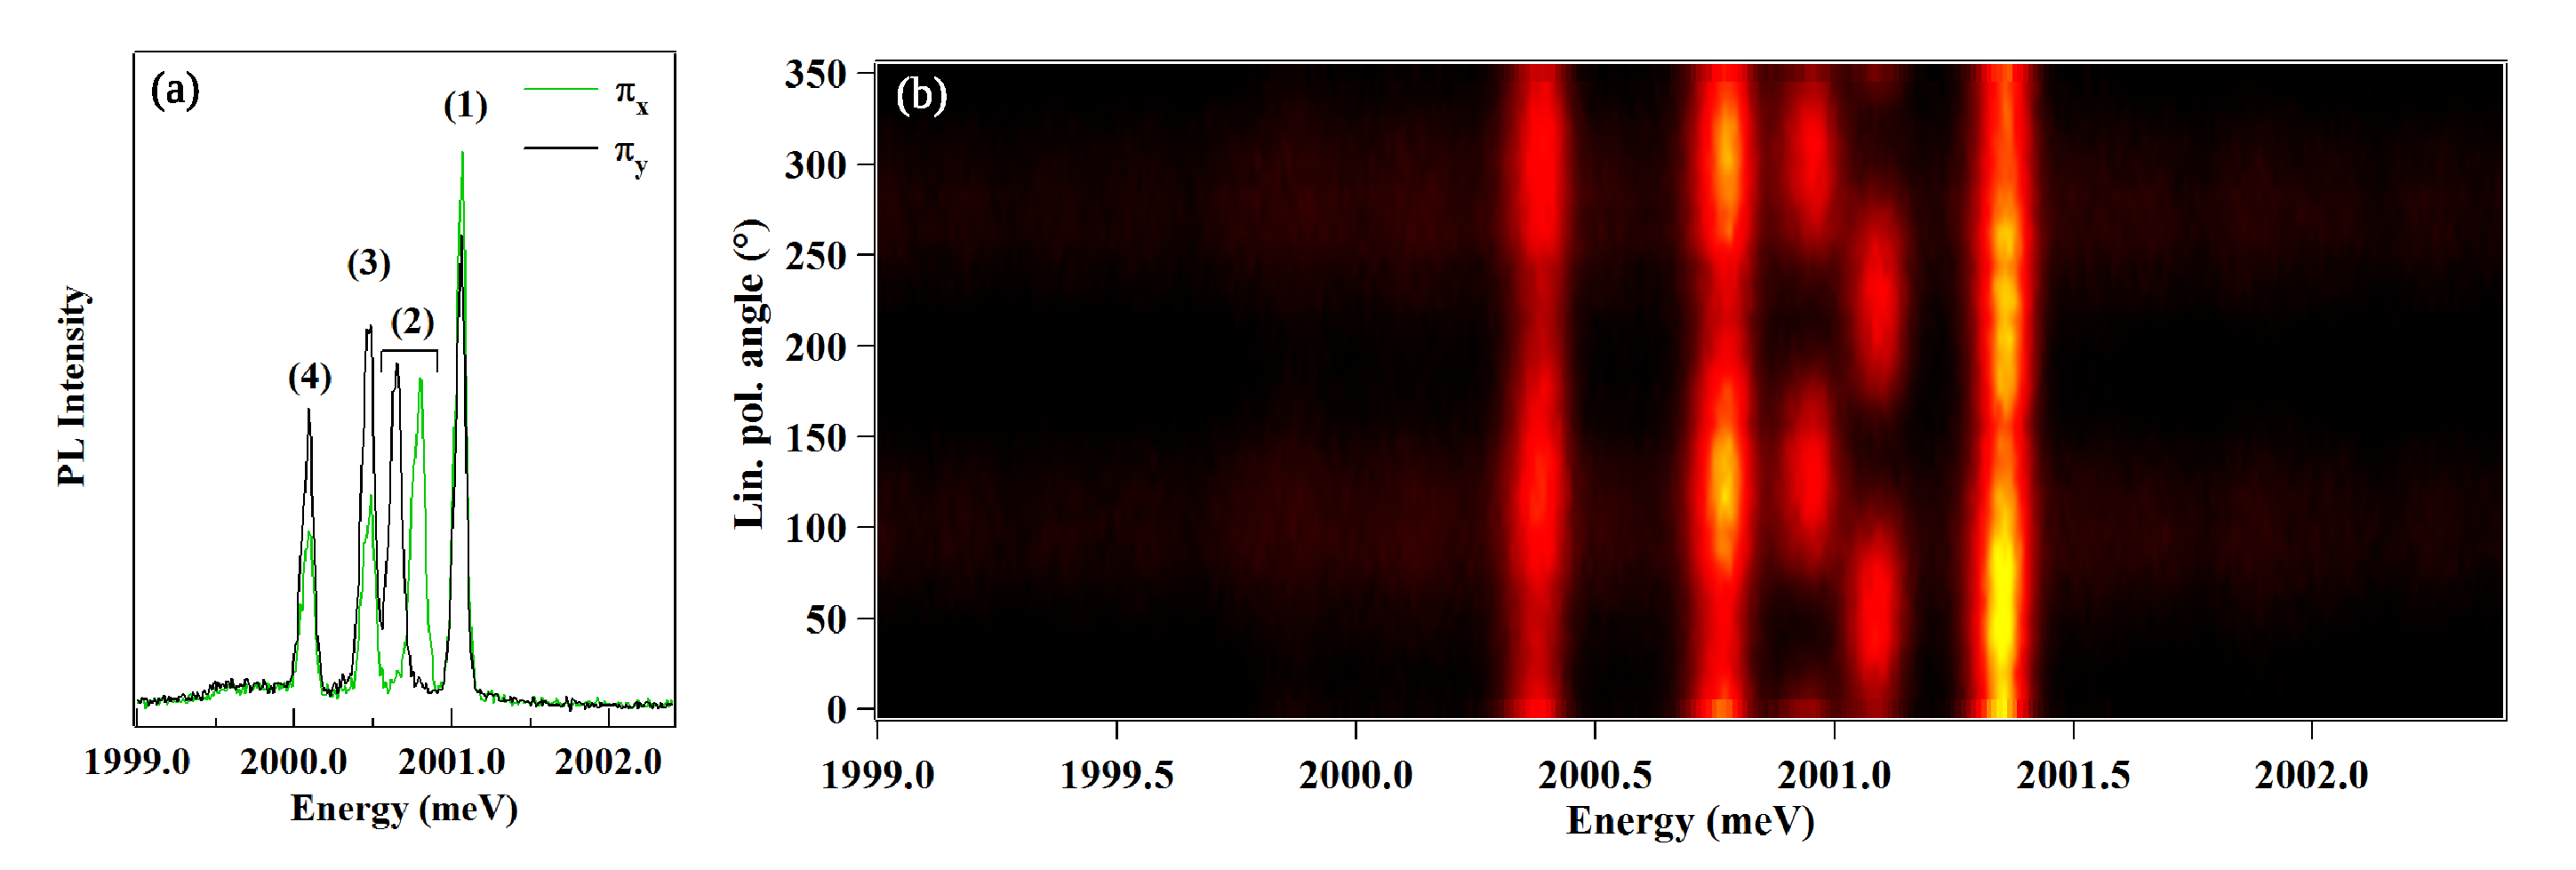
\includegraphics[width=15cm]{Picture/Fig02-LinPol.eps}
	\end{center}
	\caption{Graph in $\pi_x$ and $\pi_y$ above linear polarization of dot338 QD3
	The 0$^{\circ}$ polarization angle correspond to an emission polarized along the QD cleavage axis, either $110$ or $1\bar{1}0$.}
	\label{CrLinPolar}
	\end{figure}
	
	Cr-doped quantum dots exhibit a linear polarization dependence, as presented in Fig.~\ref{CrLinPolar}. The central line (S$_z$=0) is split and linearly polarized along two orthogonal directions. As in non-magnetic QDs, this results from a coupling of the two bright excitons $|\pm1\rangle$ by (i) the short range e-h exchange interaction in the presence of valence band mixing and/or (ii) the long-range e-h exchange interaction in a QD with an in-plane shape anisotropy~\cite{SplitInvTh}. This anisotropic e-h exchange energy mixes the bright exciton associated with the same Cr spin state, inducing an extra splitting between them. The mixing is maximum for the central pair of bright exciton (S$_z$=0) which are initially degenerated. The outer lines are also slightly linearly polarized but the influence of the e-h exchange interaction is attenuated by the initial splitting of the $|\pm1\rangle$ excitons induced by the exchange interaction with the Cr spin S$_z$=$\pm1$.	

	\begin{figure}[h!]
	\begin{center}
		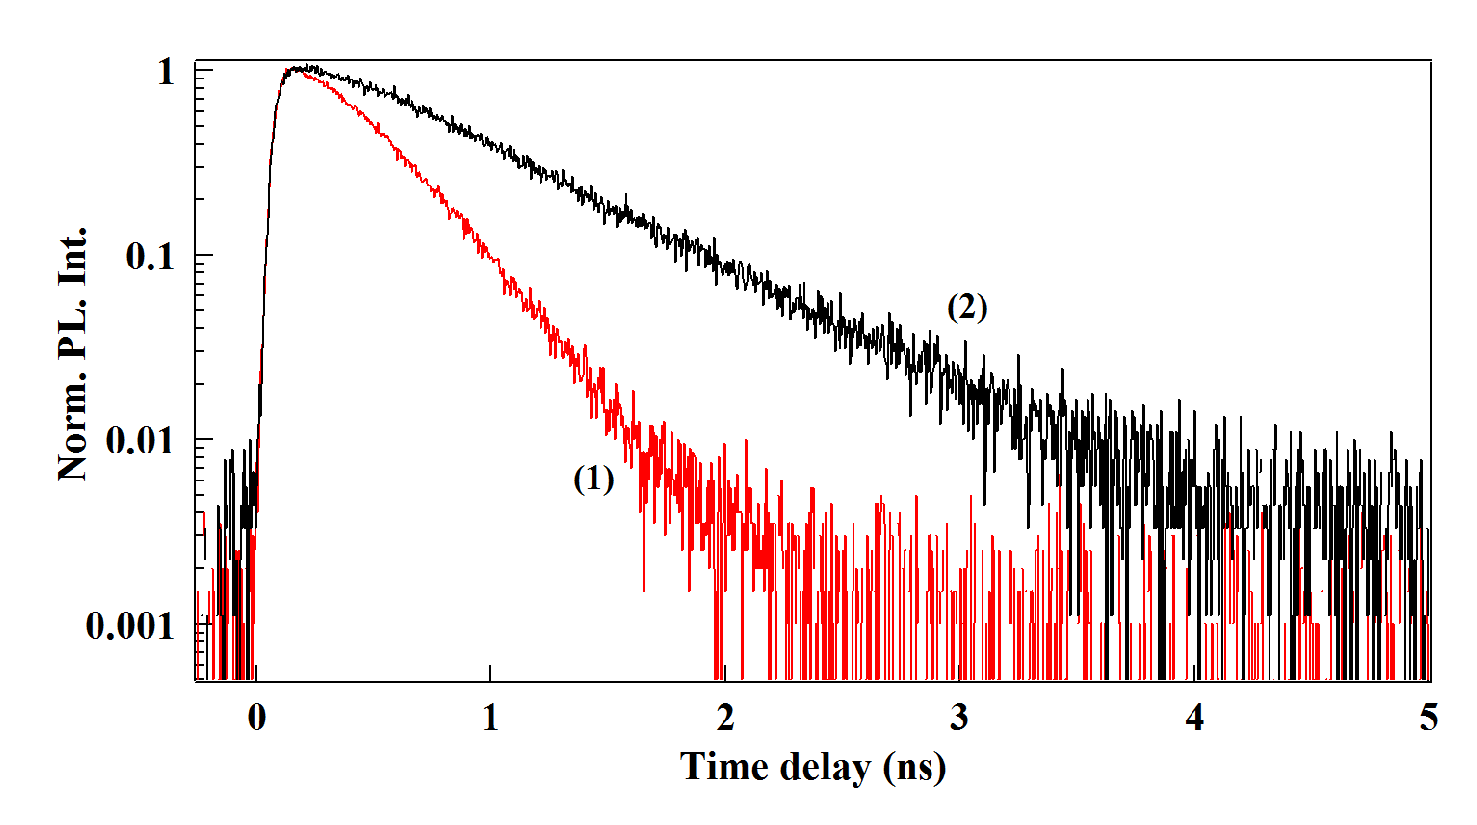
\includegraphics[width=10cm]{Picture/Fig03-Decay.eps}
	\end{center}
	\caption{Decay time on dot338 QD3}
	\label{CrDecay}
	\end{figure}

	Looking at the time resolved photoluminescence, presented in Fig.~\ref{CrDecay}, we see that the line (4) present a decay time about twice as long as the high energy peak. A long recombination time is one of the characteristics of a dark exciton emission~\cite{DELongLifetime}. Under normal circumstances, the recombination of such a state is non-radiative. However, it is possible to observe a dark exciton recombination emitting a photon in low symmetry quantum dot~\cite{DELum}. This hypothesis will be confirmed by the magneto-optical study of the dot presented in Fig.~\ref{CrMagOptExp} and \ref{CrMagOptMod}.

	\begin{figure}[h!]
	\begin{center}
		\includegraphics[width=10cm]{Picture/Fig04-EnLvl.png}
	\end{center}
	\caption{Overall energy structure (with +/- 2 with no luminescence)
	FAIRE UN PNG}
	\label{CrEnergyStruct}
	\end{figure}

	In a II-VI semiconductor, the orbital momentum of the Cr connects the spin of the atom to its local strain environment through the modification of the crystal field and the spin-orbit coupling. For biaxial strain in the (001) plane, the ground state of a Cr spin is split by a strain induced magnetic anisotropy term ${\cal H}_{Cr,\varepsilon_\parallel}=D_0S^2_z$ (see chap.~\ref{CrSemiCon}). It was deduced from electron paramagnetic resonance of bulk Cr-doped CdTe that $D_0$ is positive for compressive biaxial strain~\cite{EPRCr}. In a self-assembled CdTe/ZnTe QD with large in-plane strain, the Cr spin energy levels are split with S$_z$=0 at low energy (Fig.~\ref{CrEnergyStruct}). A value of $D_0$ in the 1 meV range can be expected for a CdTe layer strained on a ZnTe substrate, as shown in chap.~\ref{CrSemiCon}.
	
	When an electron-hole (e-h) pair is injected in a Cr-doped QD, the bright excitons are split by the exchange interaction between the spins of Cr and carriers. In flat self-assembled QDs, the heavy-holes and light-holes are separated in energy by the biaxial strain and the confinement. In a first approximation, the ground state in such QD is a pure heavy-hole (J$_z$=$\pm$3/2) exciton and the exchange interaction with the Cr spin S is described by the spin Hamiltonian ${\cal H}_{c-Cr}=I_{eCr}\vec{S}\cdot\vec{\sigma}+I_{hCr}S_zJ_z$, with $\vec{\sigma}$ the electron spin and J$_z$ the hole spin operator. I$_{eCr}$ and I$_{hCr}$ are, respectively, the exchange integrals of the electron and the hole spins with the Cr spin. These exchange energies depend on the exchange constant of the $3d$ electrons of the Cr with the carriers in CdTe and on the overlap of the Cr atom with the confined carriers. The exchange interaction of the Cr spin is ferromagnetic for both electron and hole spins in common II-VI semiconductors and a typical exchange constant 4 to 5 times larger for the holes than for the electrons is also expected in CdTe~\cite{DMSCrExchInt,CdCrSExchInt}.
	
	\begin{figure}[h!]
	\begin{center}
		\includegraphics[width=7cm]{Picture/Fig05-Temp.eps}
	\end{center}
	\caption{dot338 QD3 spectra temperature evolution}
	\label{CrTemp}
	\end{figure}
	
	For highly strained CdTe/ZnTe QDs with a weak hole confinement, the strain induced energy splitting of the Cr spin $D_0S^2_z$ is much larger than the exchange energy with the confined carriers ($D_0\gg |I_{hCr}|>|I_{eCr}|$). The exchange interaction with the exciton acts as an effective magnetic field which further splits the Cr spins states S$_z$=$\pm$1 and S$_z$=$\pm$2. The resulting X-Cr energy levels are presented in Fig.~\ref{CrEnergyStruct}. The exciton recombination does not affect the Cr atom and its spin is conserved during the optical transitions. Consequently, the large strained induced splitting of the Cr spin is not directly observed in the optical spectra. However, at low temperature, the Cr spin thermalize on the low energy states S$_z$=0 and S$_z$=$\pm$1. This leads to a PL dominated by three contributions: a central line corresponding to S$_z$=0 and the two outer lines associated with S$_z$=$\pm$1 split by the exchange interaction with the carriers.
	
	Since the thermal energy do not allow the $\pm$2 level to be populated, we tried to rise the sample temperature and see if we were able to have emission corresponding to them. The results of this experiment are presented in Fig.~\ref{CrTemp}. We were able to rise the temperature up to 40K before the peak broadening arising from the interaction with phonons completely blurred the quantum dot emission. However, even at those temperatures, no emission of the $\pm$2 level was observed.
	\newline
		
	\begin{figure}[h!]
	\begin{center}
		\includegraphics[width=15cm]{Picture/Fig06-FullPLE}
	\end{center}
	\caption{PLE of dot338 QD3. Highlight on different interesting part (mail 17/02/07 – 21:12).}
	\label{CrPLE}
	\end{figure}

	The scan map itself present some other point of interest, highlighted in Fig.~\ref{CrPLE}.
	
	The first remarkable feature of this scan is the really long luminescence of the acoustic phonon replica. As shown on the zoom in Fig.~\ref{CrPLE}(b), the peaks still emit with an excitation several millielectronvolt above the line and the dot emission energy, remaining visible until 2004 meV. One can also see two sharp intensity diminutions in this emission. Mapping the intensity of this peak emission to the quantum dot spectrum (Fig.~\ref{CrPLE}(c)), it is evidenced that these diminutions occur when the laser is in resonance with a QD emission line. The absorption then preferentially occur in this resonantly excited state than in the acoustic phonon band.
	
	At higher excitation energy, several excited state appear. The first one, the one at lower energy, is around 2018.5 meV, zoomed in on Fig.~\ref{CrPLE}(d). On this excited state, each peak presents a slightly different resonant energy. One can see that the order of appearance of the two central peaks seems to be reversed compared to the external ones. This phenomenon was first observed on QDs in GaAs quantum well~\cite{FineStructSplitGaAsdots}. This indicates an inversion of the splitting due to electron-hole exchange interaction~\cite{SplitInvTh}.
	
	Another excited state can be saw at 2025 meV. This excited state occurs on a large energy band and can be linked back to an excitation to the optical phonon. Looking at the $\sigma$ polarized emission of this state (Fig.~\ref{CrPLE}(f) and (g)), we can see that this excitation present a really good spin conservation: the low and high energy peak are strongly $\sigma$ polarized, while the central peaks do not show dependency over circular polarization, like the emission of the dot when excited on an optical quasi-resonant state. 
	
	Finally, another interesting excited state appear at 2030 meV. This state present an exchange-induced splitting  different from the splitting in the quasi-resonant state. This is due to a difference in the carriers and Cr atom wavefunction overlap. One can also noticed the this state present a stronger luminescence in $\sigma_{cross}$ than in $\sigma_{co}$, [TO REDISCUSS] hinting at a spin flip of the hole before the recombination.
		
		\subsection{Deduction of the quantum dot parameters\label{QDParam}}
		
	\begin{figure}[h!]
	\begin{center}
		\includegraphics[width=15cm]{Picture/Fig07-MagOpt.eps}
	\end{center}
	\caption{Magneto-optic of dot334 QD3 and dot334 QD4 (X + X2)}
	\label{CrMagOptExp}
	\end{figure}
		
		The structure of the energy levels in Cr-doped QDs is confirmed by the evolution of the PL spectra in magnetic field, presented in Fig.~\ref{CrMagOptExp}. One can see that the Zeeman energy of the exciton under magnetic field can compensate the exciton splitting induced by the exchange interaction with the Cr~\cite{LegerQDGeomEffect}. For QD3, this results in an anti-crossing of $|+1\rangle$ and $|-1\rangle$ excitons due to the e-h exchange interaction around B$_z$=6 T observed both in $\sigma$+ and $\sigma$- polarizations (anti-crossing (2) and (3) in Fig.~\ref{CrMagOptExp}(a)).
		
		The low energy emission presented as a dark exciton in Fig.~\ref{CrDecay} show an anti-crossing with the bright excitons under B$_z$ in $\sigma$- polarization (anti-crossing (4) in Fig.~\ref{CrMagOptExp}). As illustrated in Fig.~\ref{CrMagOptMod}(c) this anti-crossing arises from a mixing of the bright and dark excitons interacting with the same Cr spin state. Observed in $\sigma$- polarization, it corresponds to the mixing of the exciton states $|-1\rangle$ and $|+2\rangle$ coupled to the Cr spin S$_z$=-1. This dark/bright exciton coupling $\delta_{12}$ is induced by the e-h exchange interaction in a confining potential of reduced symmetry (lower than C$_{2v}$)~\cite{DERecombTh}. In such symmetry, the dark excitons acquire an in-plane dipole moment which lead to possible optical recombination at zero magnetic field~\cite{DELum} as observed in these QDs. The oscillator strength of this "dark exciton" increases as the initial splitting between $|-1\rangle$ and $|+2\rangle$ excitons is reduced by the magnetic field (Fig.~\ref{CrMagOptMod}(c)).
		
		To illustrate the influence of the QD symmetry on the magneto-optical properties of X-Cr, we compare in Fig.~\ref{CrMagOptExp} the emission of two QDs with different strain state, QD1 in (a) and QD2 in (b). For QD1, the splitting of the central peak is not clear in the PL at 0T (Fig.~\ref{SpectraXX2}(a)) without the linear polarization map, while two linearly polarized peaks appears clearly in QD2 spectra. This difference in emission arise from a difference in the in-plane strain of each QD~\cite{SplitInvTh}. The dark exciton emission is also stronger in QD2, confirming a lower symmetry than QD1.
		
		Investigating both the biexciton and the exciton in the same Cr-doped QD, we can also analyze the impact of the carrier-Cr interaction on the fine structure of the Cr spin. The magnetic field dependence of X$^2$-Cr and X-Cr emissions in QD4 are presented as a contour plot in Fig.~\ref{CrMagOptExp}(b) and (c) respectively. The PL under magnetic field of X-Cr and X$^2$-Cr present a mirror symmetry. In particular, the dark/bright exciton mixing observed around B$_z$=2.5T on the low energy side of the PL in $\sigma-$ polarization for X-Cr is observed on the high energy side in $\sigma+$ polarization for X$^2$-Cr (circles in Fig.~\ref{CrMagOptExp}(b) and (c)).
		
		If one consider the ground state of X$^2$ as a spin-singlet (total spin 0), it cannot be split by the magnetic field or the spin interaction part of the carriers-Cr Hamiltonian. The creation of two excitons in the QD cancels the exchange interaction with the Cr atom. Thus, the PL of  X$^2$-Cr is controlled by the final state of the optical transitions, i.e. the eigenstates of X-Cr, resulting in the observed mirror symmetry in the PL spectra. However, in some of the QDs, the X$^2$-Cr emission slightly deviates from this simple picture: a smaller energy splitting is observed for X$^2$-Cr compared to X-Cr (see X-Cr and X$^2$-Cr in Fig.~\ref{SpectraXX2} and Fig.~\ref{CrMagOptExp}). This shows that there is an interaction of X$^2$ with the Cr atom. It could result from a perturbation of the carriers' wave function by the interaction with the magnetic atom~\cite{CarInSpinSplit,BiexFinStruct} or a modification the local electric field which controls the Cr fine structure. [TO BE INVESTIGATED]
		
	\begin{figure}[h!]
	\begin{center}
		\includegraphics[width=15cm]{Picture/Fig08-SimulMagOpt.eps}
	\end{center}
	\caption{Linear PL + magneto-optics with modelisation and explanation of anti-crossing
	The 0$^{\circ}$ polarization angle correspond to an emission polarized along the $100$ axis.}
	\label{CrMagOptMod}
	\end{figure}
	
	We calculated the magneto-optic behaviour of Cr-doped QDs by diagonalizing the complete Hamiltonian of the e-h-Cr system presented in chap.~\ref{DMSQDTh}. We considered the general case of QDs with a symmetry lower than C$_{2v}$ (truncated ellipsoidal lens for instance~\cite{DERecombTh}), and took into account the influence of this reduced symmetry on the valence band and on the e-h exchange interaction. The population of the X-Cr spin states split by the large magnetic anisotropy and the carriers-Cr exchange interaction is described by a spin effective temperature T$_{eff}$. The results of the model obtained with T$_{eff}$=25K, D$_0$=2.5 meV and an electron-Cr (hole-Cr) exchange interaction I$_{eCr}$=-70$\mu$eV (I$_{hCr}$=-280 $\mu$eV) are reported in Fig.~\ref{CrMagOptMod}(parameters not specific to Cr-doped QDs are listed in Tab.~\ref{CrModelParam}). Such parameters do not aim to fit the data and are only reasonable order of magnitude. The PL of X-Cr at zero field and its evolution in magnetic field can be qualitatively reproduced. In particular, the description of the spin states occupation by T$_{eff}$ is sufficient to reproduce the observed emission from the three low energy X-Cr levels (Cr spin states S$_z$=0 and S$_z$=$\pm$1). The splitting of the central line at zero field (anti-crossing (1)) and the anti-crossings under magnetic field (anti-crossings (2) and (3) around B$_z$=6T for the Cr spin states S$_z$=+1 and anti-crossings (4) with the dark exciton around B$_z$=2T) are also well reproduced by the model.
	
	\begin{table}[t]
	\caption{Values of the parameters used in the model of Cr-doped CdTe/ZnTe quantum dot presented in Fig.~\ref{SpectraXX2}(b). The value of the parameters not listed in the table is 0. The chosen values are typical for CdTe/ZnTe quantum dots and can be compared with parameters extracted from Mn-doped quantum dots \cite{DynhMn,VBM}. These values are reasonable to reproduce the emission of the QDs presented in this thesis.}
	\renewcommand{\arraystretch}{1.0}
	\begin{tabular}{p{0.9cm}p{0.9cm}p{0.9cm}p{0.9cm}p{0.9cm}p{0.7cm}p{1.3cm}p{1.3cm}p{0.9cm}p{0.9cm}p{0.9cm}}
\hline\hline
I$_{eCr}$ & I$_{hCr}$ & $\delta_0$ & $\delta_1$ & $\delta_{12}$ & $\delta_{11}$ & $\frac{Module(Q)}{\Delta_{lh}}$ & $\frac{Module(R)}{\Delta_{lh}}$ & arg(R) & $D_0$ & $g_{Cr}$ \\
$\mu eV$ & $\mu eV$ & $meV$ & $\mu eV$ & $\mu eV$ & $\mu eV$ &  & & & $meV$ &  \\
\hline
-70 & -280 & -1 & 250 & 150 & 50 & 0.05 & 0.05& $-\frac{\pi}{2}$ & 2.5 & 2 \\
\hline\hline
	\end{tabular}
	\begin{tabular}{p{0.9cm}p{0.9cm}p{1.3cm}p{0.9cm}p{0.9cm}}
\hline\hline
$g_{e}$ & $g_{h}$ & $\gamma$ & $\eta$ & $T_{eff}$ \\
  &  & $\mu eV/T^2$ & $\mu eV$ & K \\
\hline
-0.7 & 0.4 & 1.5 & 25 & 25 \\
\hline\hline	  
	\end{tabular}
	\label{CrModelParam}
	\end{table}
	
	The magnetic anisotropy D$_0$ cannot be precisely extracted from the PL spectra. However, a too large value would produce a smaller PL intensity of the sates S$_z$=$\pm$1 than observed experimentally. In addition, for D$_0$ $<$ 2.25 meV, an anti-crossing due to an electron-Cr flip-flop controlled by I$_{eCr}$, labelled (5) in Fig.~\ref{CrMagOptMod}(c), would appear below B$_z$=11T on the central line in $\sigma$+ polarization.
	\newline
	
	\begin{figure}[h!]
	\begin{center}
		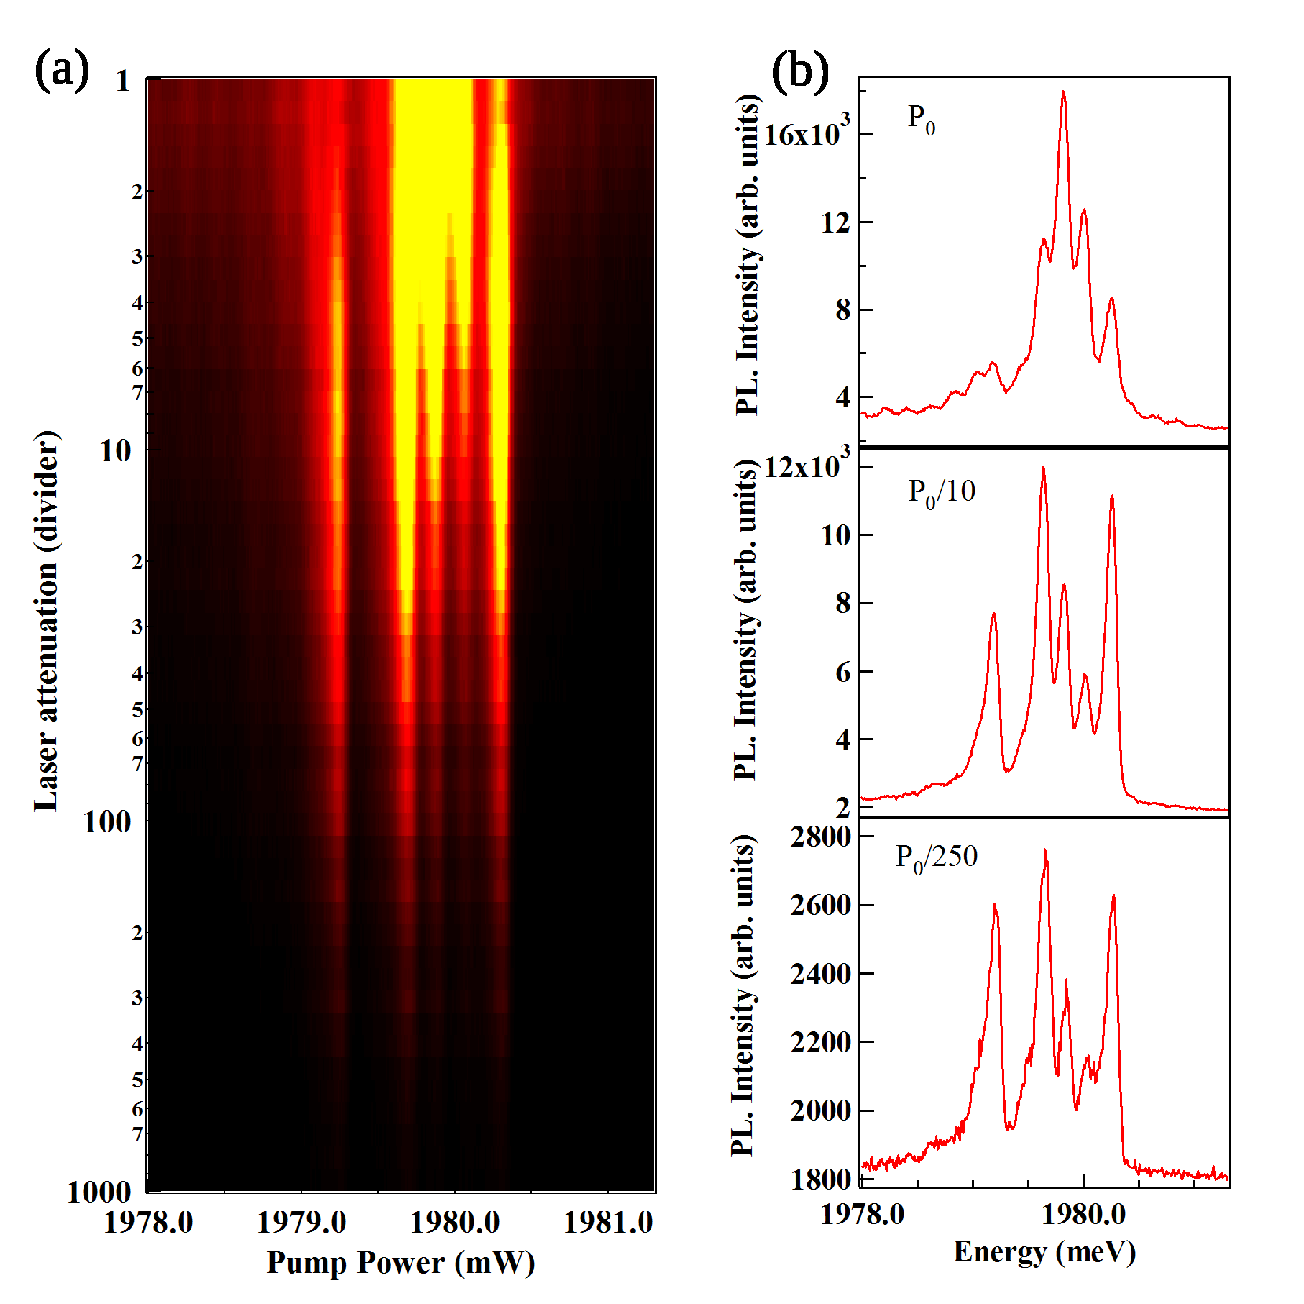
\includegraphics[width=10cm]{Picture/Fig09-PwVar.eps}
	\end{center}
	\caption{Excitation power variations on dot334 QD3 and plot of the intensity of each peak}
	\label{CrSpectraPwExp}
	\end{figure}
	
	Another source of informations on the system is its evolution under excitation power. Such an experiment is reported on Fig.~\ref{CrSpectraPwExp}(a). As expected, the PL is becoming more intense with the augmentation of the excitation laser, since more exciton are produced and thus injected in the quantum dot. However, this power augmentation response is not the same for each of the peaks. The two central peaks, associated with the $|0\rangle$ states, start at about twice the intensity of the $|\pm1\rangle$ peaks for the most intense one, seemingly never reaching their maximum under our power range. However, when lowering the excitation power, they diminish quickly, and even seems to disappear at low energy, when exterior peaks still show luminescence. Plotting this evolution shows that the two central peaks exhibit a super-linear evolution. On the other side, the exterior peaks begin by rising in intensity before diminishing in a sub-linear fashion. This is coherent with the usual picture, where high power populating preferentially X$^2$-Cr states, while low power populates preferentially X-Cr states~\cite{??}. Finally, one can notice that the dark exciton exhibit the same behaviour, but the maximum emission intensity is at slightly lower power than the $|\pm1\rangle$.

	\begin{figure}[h!]
	\begin{center}
		\includegraphics[width=10cm]{../FillingPicture.png}
	\end{center}
	\caption{Power variation simulation}
	\label{CrSpectraPwMod}
	\end{figure}
	
	The results of this evolution are well reproduced by our spin effective Hamiltonian, using the parameters found for the dot from the magneto-optics and the linear polarization fitting. The model results are presented in Fig.~\ref{CrSpectraPwMod}. [NOT SURE, TO BE REDISCUSSED]The super-linear behaviour of the central peaks can be explained by the proximity of dark exciton states. High power excitation can unlock radiative recombination path to states remaining nonradiative at low excitation power~\cite{PwSuperLinInc}. Such states linked to the $|0\rangle$ state make the emission on its peaks present a super-linear behaviour when excited at high power. 
	
	\begin{figure}[h!]
	\begin{center}
		\includegraphics[width=10cm]{Picture/Fig11-HighE.eps}
	\end{center}
	\caption{Linear polar and magneto-optics simulation with high E}
	\label{CrHighE}
	\end{figure}
	
	One characteristic emerging from our model is the necessity to have a E value close to 0 $\mu$eV to reproduce the measures. Now that we show that our model reproduce well the evolution of the emission under various type of excitation, we can run it to see the influence of E on the emission. Results of such a study are presented on Fig.~\ref{CrHighE}, (a) and (b) for the X-Cr system, and (c) and (d) for the X$^c$-Cr one. This simulation was done by applying a small magnetic anisotropy along the X axis of the quantum dot (D$_x$ = 50 $\mu$eV, D$_y$ = 0 $\mu$eV, to be compared with D$_z$ = 2500 $\mu$eV), creating an effective E from this strain anisotropy in the QD plane.
	
	The first remarkable feature appear on the linear polarization dependency of the X-Cr system(Fig.~\ref{CrHighE}(a)). While, with a small value of E, only the $|0\rangle$ states presents linear polarization, at higher value, $|\pm 1\rangle$ states also present some. The quantum dot should then appears to present six peaks when probed in circular polarization. As expected, even with this high E value, X$^c$-Cr doesn't present any linear polarization dependency, as shown on Fig.~\ref{CrHighE}(c), and would in this case still present the usual three peaks structure.
	
	The evolution of the emission under magnetic field also presents different characteristics than a QD with magnetic anisotropy purely along z. Fig.~\ref{CrHighE}(b) presents the evolution in B of the X-Cr emission. Firstly, one can see anti-crossings at $\pm$5T appearing on both $|+1\rangle$ and $|-1\rangle$, and not only one of them. Moreover, around 0T, several anti-crossing appear, not only on the $|0\rangle$ peak, but also on the $|\pm1\rangle$. X$^c$-Cr also presents a peculiar magnetic field evolution in a QD with a E value, presented in Fig.~\ref{CrHighE}(d). If, for high B, no anti-crossing is visible, one s around 0T. This anti-crossing appears when the Zeeman effect of the Cr atom compensates the electron-Chromium interaction and the hole-Chromium interaction. Such an anti-crossing is characteristic of this type of dots and will be useful in their identification: while the six peaks of the X-Cr might be undistinguishable at 0T, X$^c$-Cr would still present 3 peaks and show this particular evolution under magnetic field.

				
	
	\section{The case of six peaks dots}
	
	We showed in the section \ref{QDParam} that each emission can be doubled for a QD with a a non-null in-plane anisotropy, each of these peaks having dependency in linear polarization. Some dots present this structure, but their evolution in magnetic field didn't show any anti-crossing. Such a dot is presented in Fig.~\ref{CrSixPeaksMagOpt}.
	
	\begin{figure}[h!]
	\begin{center}
		\includegraphics[width=15cm]{Picture/Fig12-6peaks.eps}
	\end{center}
	\caption{dot334 QD150521/22 and dot390 QD14 spectra + dot334 QD150521/22 and dot390 QD14 linear pol + dot334 QD150521/22 magneto-optics}
	\label{CrSixPeaksMagOpt}
	\end{figure}
	
	A common feature of all of these dot is the well defined X$^c$-Cr structures emission, shown on Fig.~\ref{CrSixPeaksMagOpt}(a) between 1946meV (X$^-$-Cr) and 1950mev (X$^+$-Cr). Such QDs always present thin and well splitted X$^c$-Cr emission peaks. X-Cr and X$^2$-Cr appear in two different forms in $\sigma$ polarization detection. In Fig.~\ref{CrSixPeaksMagOpt}(a), we can see these two structures appearing with three well defined peaks, with a broad emission. The second type of emission observed is presented in Fig.~\ref{CrSixPeaksMagOpt}(c). One can see the three peaks are no longer distinguishable, only a broad emission band is measured at their positions. However, when detecting in $\pi$ polarization (Fig.~\ref{CrSixPeaksMagOpt}(b) and (d)), both present the same structure: six peaks with linear polarization dependency.
	
	This figure would be coherent with a QD presenting a strong in-plane anisotropy. To analyse them further, magneto-optic experiments were performed on these dots. The result of such an experiment is presented in Fig.~\ref{CrSixPeaksMagOpt}(e). The shift induced by the diamagnetic shift and the Zeeman is clearly visible. However, no anti-crossing appears whatever the magnetic field applied. As shown in Fig.~\ref{CrHighE}, QD with a high in-plane anisotropy should present several anti-crossing, especially around 0T. The picture is then not coherent with these low symmetry quantum dots.
	
	\begin{figure}[h!]
	\begin{center}
		\includegraphics[width=5cm]{Picture/Fig13-EfieldXc.png}
	\end{center}
	\caption{dot390 QD4 electric field map zoom on X+-Cr}
	\label{CrSixPeaksEFieldX+}
	\end{figure}
	
	In order to have more informations on these dots, it was decided to study them applying a bias voltage. In order to apply an electric field, we realized a sample with a Schottky gate in the same fashion as the one in chap.~\ref{ChargeSelec}. The resulting map is presented in Fig.~\ref{CrSixPeaksEFieldX+}. The first visible feature is the strong electric field dependency of the emission energy, more marked for X-Cr than for the X$^c$-Cr systems. The emission energy variation of the X-Cr complex occur on a 2.9 meV scale.
	
	There is another remarkable point on these maps, evidenced on the X$^+$-Cr complex on the Fig.~\ref{CrSixPeaksEFieldX+}(b): the splitting between each peak is changing with the applied electric field. The emission extension varies from 0 meV for an applied bias voltage of -12V (no splitting) to 0.76 meV for 13V applied. This disappearance of the splitting for a certain bias voltage indicates that the overlap between the electron and the hole wave functions is changed by the application of an exterior electric field, to the point where they don't overlap at all.

	\begin{figure}[h!]
	\begin{center}
		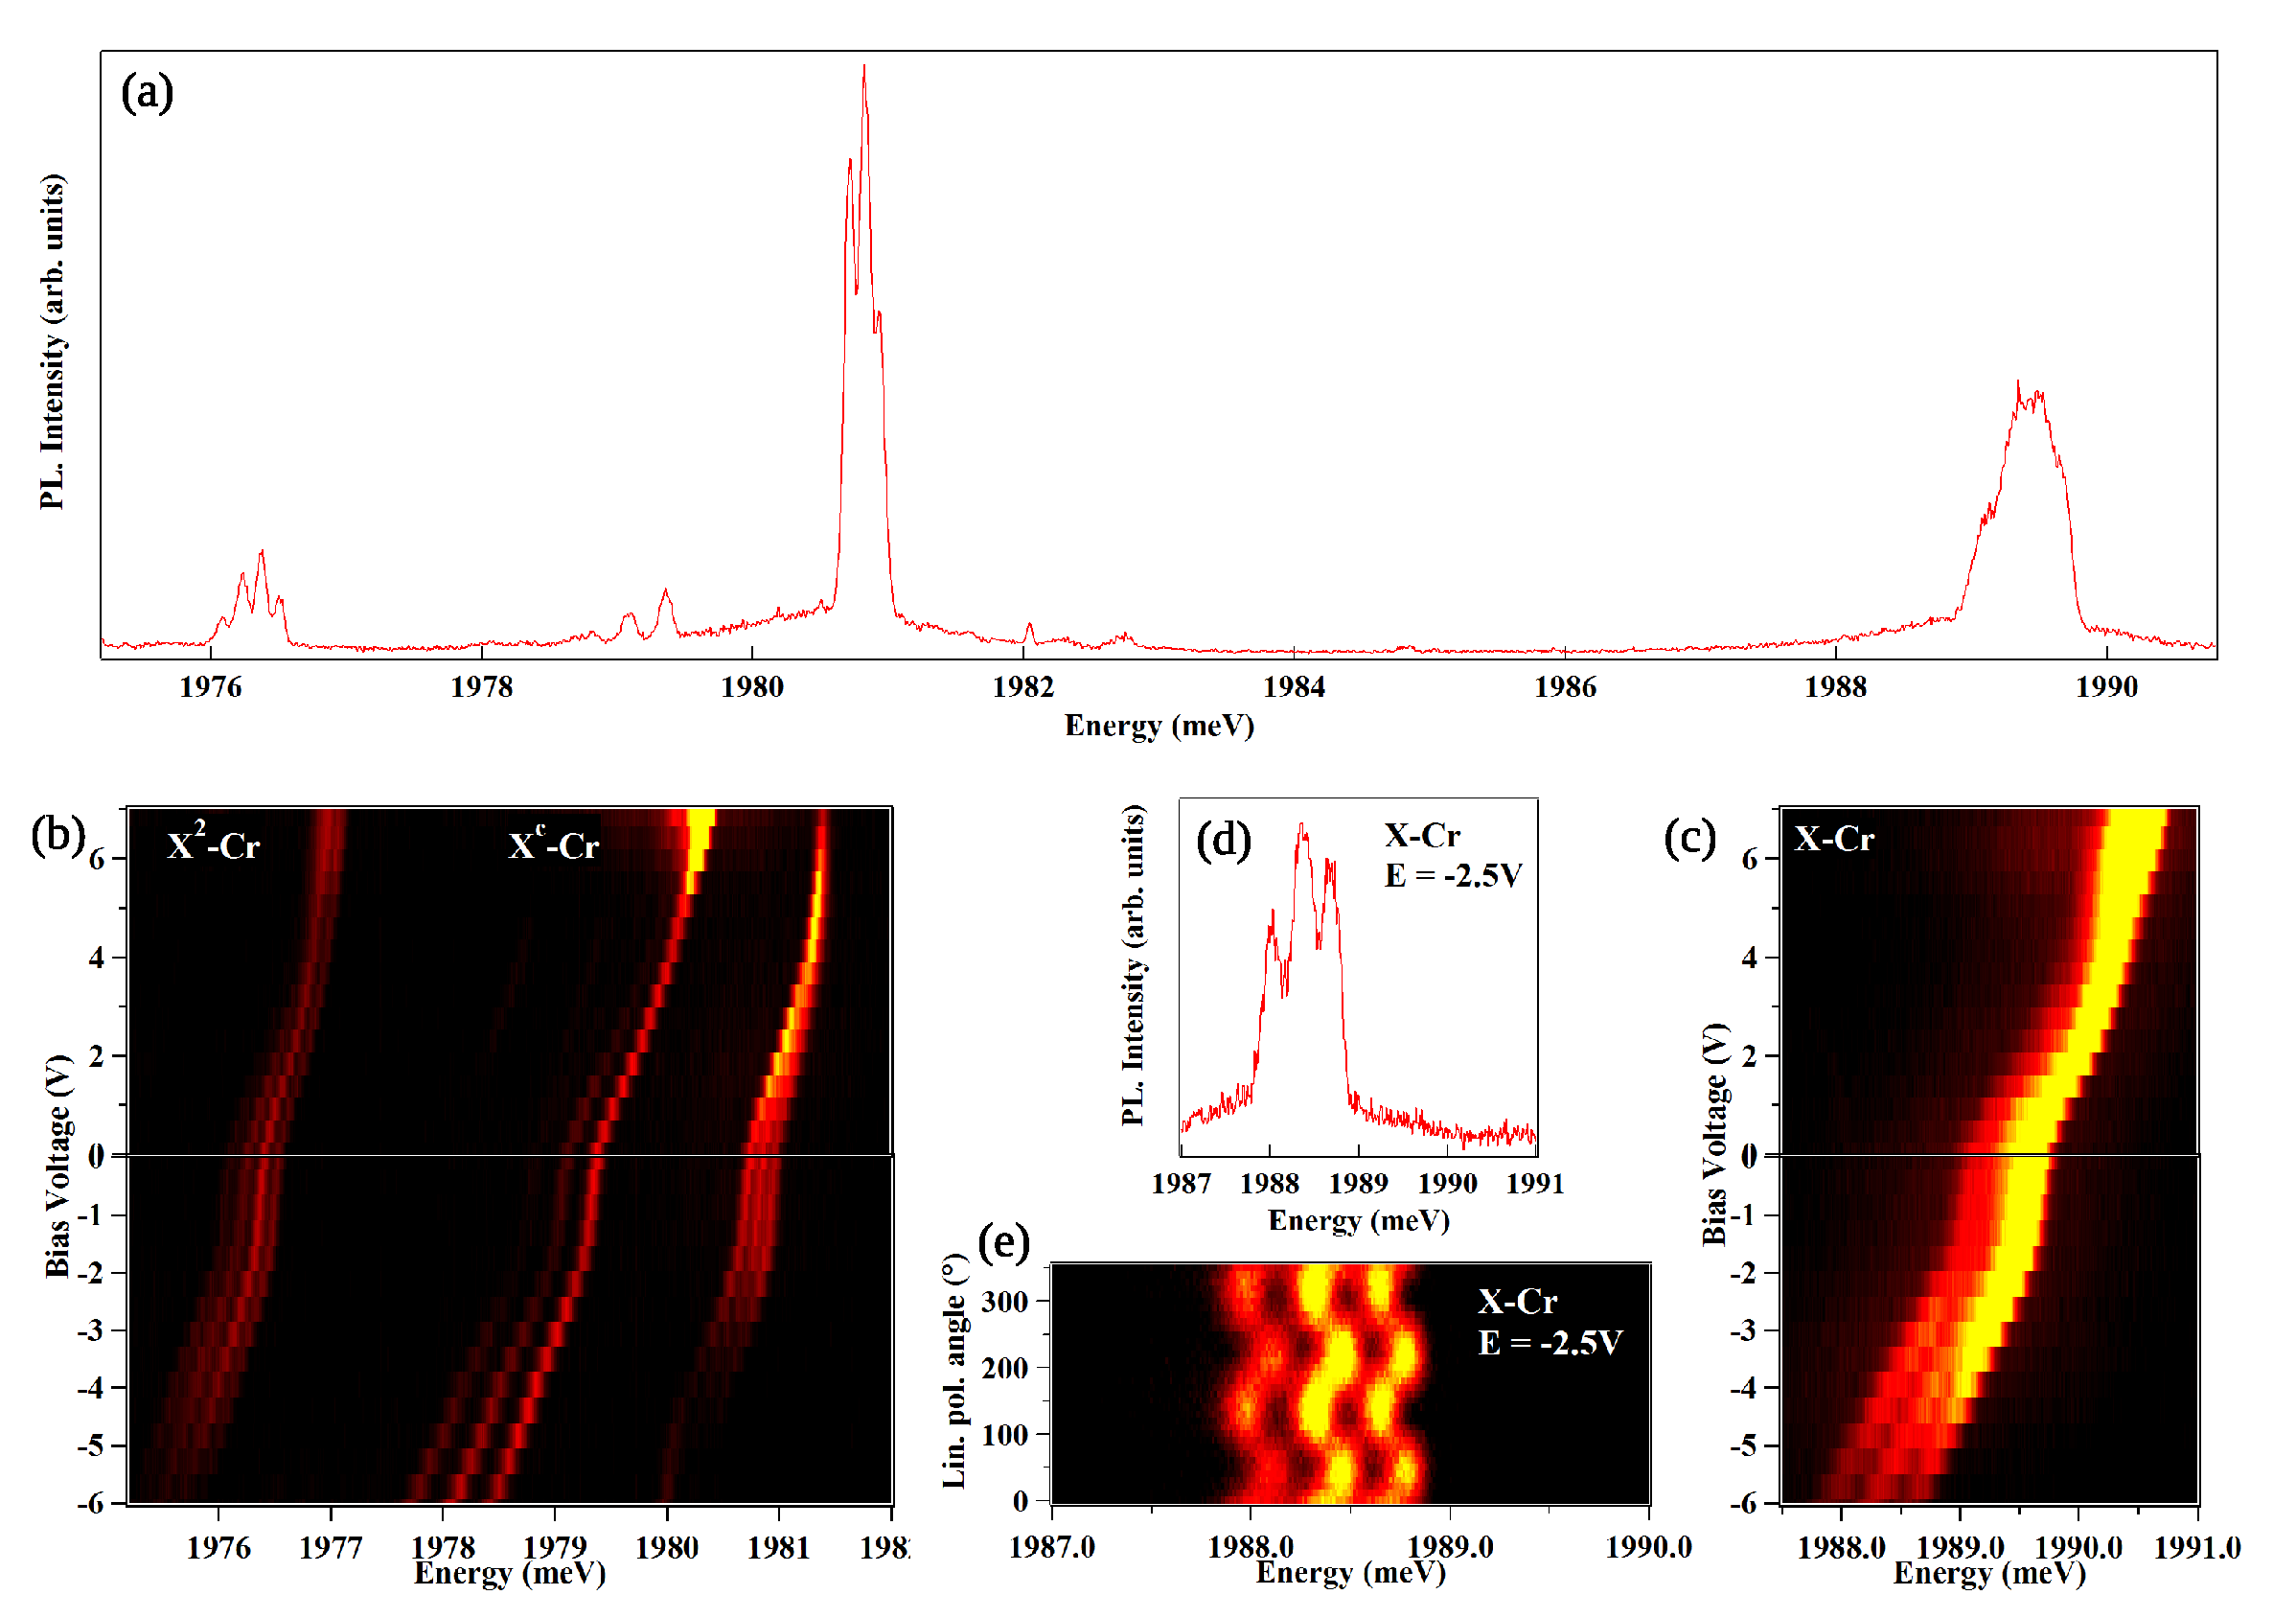
\includegraphics[width=15cm]{Picture/Fig14-SplitUnderEfiled.eps}
	\end{center}
	\caption{dot390 QD14 map under E field (cut at -4V) + spectra at E = -2.5V and E = 0V + linear polar at E = -2.5V and E = 0V}
	\label{CrSixPeaksComplete}
	\end{figure}
	
	Fig.~\ref{CrSixPeaksComplete}(a) shows that, using electric field, we can manipulate the splitting of any given state. For all positive bias voltage between 0V and 13V, X-Cr present a broad emission containing all six peaks in linear emission, as show on Fig.~\ref{CrSixPeaksComplete}(d). The splitting begins to clearly appears around an applied voltage of -1V. X$^+$-Cr presents a splitting at 0V, widening at lower applied electric field, and diminishing when going to positives, with null splitting at 2.5V. The same kind a phenomena are also visible on X$^-$-Cr and X$^2$-Cr.
	
	\begin{figure}[h!]
	\begin{center}
		\includegraphics[width=10cm]{../FillingPicture.png}
	\end{center}
	\caption{Cr accessible states in ZnTe + Schema on action of punctual charge on the wave function + the application of an electric on such a system}
	\label{CrOutsideDot}
	\end{figure}
	
	
	This three peaks emission shows that we have a three levels system emitting at three different energies. However, the magnetic field evolution presented in Fig.~\ref{CrSixPeaksMagOpt}(e) does not reflect the presence of a magnetic atom in the quantum dot. Moreover, evolution under electric field shows huge changes in the wave function overlap. Finally, the bias voltage shows a strong shift under the application of an electric field.
	
	Quantum dots with multiple energy emission was already found, linked to a change of the QD electrical environment, like the proximity of a defect with two possible states (neutral or charged). This system can then emit at two different energies, depending on the defect charge state, changing over time~\cite{??}. A defect with three charged states could then create three emission peaks. 
	
	Cr in ZnTe is incorporated as Cr$^{2+}$, but, as shown on Fig.\ref{CrOutsideDot}(a), the Cr$^+$ and Cr$^3+$ are also accessible~\cite{CrZnTe}, meaning all three electric states are accessible, either by capting an electron (Cr$^+$) or a hole (Cr$^3+$). Considering such a charge close to the QD, it can be view as a punctual one, since the dot is far bigger than the atom. The effect on the wave functions, presented in Fig.\ref{CrOutsideDot}(b) and (c), differs depending on the electrical charge of the Cr atom, leading to three different possible emission energies.
	
	This hypothesis is currently tested, along with the capacity for the Cr to diffuse outside the quantum dots layer.

\bibliographystyle{unsrt}
\bibliography{../Bibliography}

\end{document}